\subsection{Formulating Linear Programming Problems}
	\begin{ex}{The Diet Problem}{label}
		A student is subject to the following dietary requirements,

		\vphantom{.}

		\resizebox{\textwidth}{!}{
		\begin{tabular}{llllll}
		\textbf{Food} & \textbf{Energy} & \textbf{Protein} & \textbf{Calcium} & \textbf{Price} & \textbf{Servings} \\ \hline
		Porridge & 110 & 4 & 2 & 10 & 4 \\ \hline
		Chicken & 205 & 32 & 12 & 200 & 3 \\ \hline
		Eggs & 160 & 13 & 54 & 40 & 4 \\ \hline
		Milk & 160 & 8 & 285 & 35 & 8 \\ \hline
		Apple Pie & 420 & 4 & 22 & 190 & 3 \\ \hline
		Pork and Beans & 260 & 14 & 80 & 90 & 2 \\ \hline
		Requirement & 2000 & 55 & 800 & None & None \\
		\end{tabular}}

		\vphantom{.}

		\noindent The goal is to find,
		\[\min 10x_1 + 200x_2 + 40x_3 + 35x_4 + 190x_5 + 90x_6 \]
		\noindent subject to the constraints,
		\begin{align*}
			x_i \geq 0 \text{ for all $i \in [6]$} & \\
			x_1 \leq 4, x_2 \leq 3, x_3 \leq 4, x_4 \leq 8, x_5 \leq 3, x_6 \leq 2 & \\
			110x_1 + 205x_2 + 160x_3 + 160x_4 + 420x_5 + 260x_6 &= 2000 \\
			4x_1 + 32x_2 + 13x_3 + 8x_4 + 4x_5 + 14x_6 &= 55 \\
			2x_1 + 12x_2 + 54x_3 + 285x_4 + 22x_5 + 80x_6 &= 800 \\
		\end{align*}

	\end{ex}

	\begin{marginfigure}
		\begin{center}
			
\includegraphics[width=0.6\textwidth]{fig-4.png}
		\end{center}

		\noindent Any linear equation in $n$ variables defines a hyperplane in $\mathbb{R}^n$, and the intersection of a finite number of hyperplanes is called a polyhedron. By rotating the space so that the objective function points downward, any linear program is the problem of finding the lowest point in a given polyhedron.
	\end{marginfigure}

	\begin{defn}[Linear Program]
		A \textbf{linear program} minimizes or maximizes a linear objective function subject to a set of linear constraints.
	\end{defn}

	\begin{defn}[Feasibility]
		A point $x \in \mathbb{R}^n$ is \textbf{feasible} with respect to some linear program if it satisfies all of the linear constraints.
	\end{defn}

	\begin{defn}[Primal Linear Program]
		A primal linear program is,
		\[
		    \max \Set{ \sum_{j=1}^n c_j \cdot x_j \ | \begin{array}{l}
		    \sum_{j=1}^n a_{ij} \cdot x_j \leq b_j \text{ for all } i \in [m] \\
		    x_j \geq 0 \text{ for all } j \in [n]
		  \end{array}}
		\]	
	\end{defn}

	\begin{rmk}
		The matrix encoding of a linear program in standard form is,
		\[
		    \max \Set{ c^T \cdot x \ | \begin{array}{l}
		    Ax \leq b \\
		    x \geq 0
		  \end{array}}
		\]	
	\end{rmk}

	\begin{ex}{Standard Form}{label}
		Any linear program can be converted into standard form,
		\[
		\begin{array}{ll}
		\operatorname{maximise} & \sum_{j=1}^{n} c_{j} x_{j} \\
		\text { subject to } & \sum_{j=1}^{n} a_{i j} x_{j} \leq b_{i} \quad \forall i \in[m] \\
		& x_{j}  \geq 0  \quad \forall j \in[n]
		\end{array}
		\]
		\begin{itemize}
			\item For each variable $x_j$, add:
				\begin{itemize}
					\item Two new variables $x_i^+, x_i^-$
					\item Recover $x_j$ by taking, $x_j = x_j^+ - x_j^-$
					\item Inequalities, $x_j^+ \geq 0$ and $x_j^- \geq 0$
				\end{itemize}
			\item Replace any equality constraint $\sum_j a_{ij}x_j = b_i$ with:
				\begin{itemize}
					\item An inequality constraint, $\sum_j a_{ij}x_j \geq b_i$
					\item An inequality constraint $\sum_j a_{ij}x_j \leq b_i$
				\end{itemize}
			\item Replace any upper bound constraint $\sum_j a_{ij}x_j \geq b_i$ with,
					\begin{itemize}
						\item The equivalent lower bound, $\sum_j -a_{ij}x_j \leq -b_i$
					\end{itemize}
			\end{itemize}
	\end{ex}

		\begin{defn}[Dual Linear Program]
			For every primal linear program,
			\[
			\begin{array}{lrlr}
			\operatorname{maximize} & \sum_{j=1}^{n} c_{j} \cdot x_{j} & & \\
			\text { subject to } & \sum_{j=1}^{n} a_{i j} \cdot x_{j} & \leq b_{i} &\forall i \in[m] \\
			& x_{j} & \geq 0 & \forall j \in[n]
			\end{array}
			\]
			\noindent there is a corresponding \textbf{dual linear program},
			\[
			\begin{array}{lrlr}

			\operatorname{minimize} & \sum_{i=1}^{m} b_{i} \cdot y_{i} & & \\
			\text { subject to } & \sum_{i=1}^{m} a_{i j} \cdot y_{i} & \geq c_{j} & \forall j \in[n] \\
			& y_{i} & \geq 0 & \forall i \in[m]
			\end{array}
			\]
			 that can be obtained by swapping the constraints and the variables.
		\end{defn}

		\begin{rmk}
			The matrix encoding of the dual linear program is,
			\[
		    \min \underbrace{\Set{ b^Ty \ | \begin{array}{l}
		    A^T y \geq c \\
		    y \geq 0
		  \end{array}}}_{Dual}
			\iff
			\max \underbrace{\Set{ c^Tx \ | \begin{array}{l}
		    Ax \leq b \\
		    x \geq 0
		  \end{array}}}_{Primal}
		\]	
		\end{rmk}

	\begin{defn}[Dictionaries]
		Given a linear program in standard form,
		\[
		    \max \Set{ \sum_{j=1}^n c_j \cdot x_j \ | \begin{array}{l}
		    \sum_{j=1}^n a_{ij} \cdot x_j \leq b_j \text{ for all } i \in [m] \\
		    x_j \geq 0 \text{ for all } j \in [n]
		  \end{array}}
		\]	
		\noindent we introduce \textbf{slack variables}\footnote{Slack variables are variables that has been introduced to turn an inequality constraint into an equality constraint.} $x_{n+1}, x_{n+2}, \cdots, x_{n + m}$,
		\[x_{n+i} = b_i - \sum_{j=1}^n a_{ij} \cdot x_j \quad \text{for $i \in [m]$ and } \quad z = \sum_{j=1}^n c_j \cdot x_j \]
		\noindent and denote the objective function by $z$.
	\end{defn}

	\begin{defn}[Basic Variable]
		\textbf{Basic} variables are the variables that appear on the left-hand side of a dictionary, and they constitute a basis.
	\end{defn}

	\begin{defn}[Nonbasic Variable]
		\textbf{Nonbasic} variables are the variables that appear on the right-hand side of a dictionary.
	\end{defn}

	\begin{rmk}
		Dictionaries define basic variables in terms of non-basic ones.
	\end{rmk}

	\subsection{The Simplex Algorithm: Method}
	\begin{defn}[Simplex Algorithm]
		The \textbf{simplex algorithm} works as the Gauss-Jordan elimination method on inequalities and constraints,
		\begin{itemize}
			\item Represent the linear program in slack form
			\item Convert one slack form into an equivalent slack form, ensuring that the value of the objective function does not decrease while likely increasing it
			\item Repeat until the optimal solution becomes apparent
		\end{itemize}
	\end{defn}

	\begin{ex}{Slack Variables}{label}
		Take the linear program, 
		\[
		\begin{array}{cl}
		\operatorname{maximize} & 5 x_{1}+4 x_{2}+3 x_{3} \\
		\text { subject to } & 2 x_{1}+3 x_{2}+x_{3} \leq 5 \\
		& 4 x_{1}+x_{2}+2 x_{3} \leq 11 \\
		& 3 x_{1}+4 x_{2}+2 x_{3} \leq 8 \\
		& x_{1}, x_{2}, x_{3} \geq 0
		\end{array}
		\]
		\noindent Write it in dictionary form,

		\vphantom{.}

		\begin{center}
		\begin{tabular}{lllllllll}
		$z$   & = &    &     & $5x_1$ & $+$ & $4x_2$ & $+$ & $3x_3$ \\ \hline
		$x_4$ & = & 5  & $-$ & $2x_1$ & $-$ & $3x_2$ & $-$ & $x_3$  \\
		$x_5$ & = & 11 & $-$ & $4x_1$ & $-$ & $x_2$  & $-$ & $2x_3$ \\
		$x_6$ & = & 8  & $-$ & $3x_1$ & $-$ & $4x_2$ & $-$ & $2x_3$
		\end{tabular}
		\end{center}

		\vphantom{.}

		\noindent and restate our problem as,
		\[
		\begin{array}{cl}
		\operatorname{maximize} & z \\
		\text { subject to } & x_{1}, x_{2}, x_{3}, x_{4}, x_{5}, x_{6} \geq 0
		\end{array}
		\]
	\end{ex}

	\begin{ex}{The Simplex Algorithm}{label}
	The \textbf{feasible solution} that is implicit in our dictionary is,
	\[(x_1, x_2, x_3, x_4, x_5, x_6) = (0,0,0,5,11,8)\]

	This gives an \textbf{objective value} of,
	\[z = 5x_1 + 4x_2 + 3x_3 = 0\]

	In the first iteration, we attempt to increase the value of $z$ by making one of the right-hand side variables positive.
	\end{ex}

	\begin{marginfigure}
		\textbf{Linear Programming Algorithms:}
		\begin{itemize}
			\item \textit{Simplex Algorithm.} In the feasible region, $x$ moves from vertex to vertex in the direction of $c$. The algorithm is simple, but runs in exponential time in the worst case.
			\item \textit{Ellipsoid Algorithm.} The algorithm begins with an ellipsoid that includes the optimal solution, and continues to shrink the ellipsoid until the optimal solution is found.
			\item \textit{Interior Point Method.} $x$ moves inside the polytope following $c$.
		\end{itemize}
	\end{marginfigure}

	\begin{defn}[Entering Variable]
		The \textbf{entering variable} at each iteration is the nonbasic variable that enters the basis to increase $z$\footnote{We may choose any nonbasic variable with a positive coefficient in the top row of the dictionary.}. 
	\end{defn}

	\begin{defn}[Leaving Variable]
		The \textbf{leaving variable} at each iteration is the variable that is removed from the basis for the entering variable\footnote{We may choose any basic variable whose non-negativity imposes the most stringent upper bound on the increment of the entering variable.}. 
	\end{defn}

	\begin{ex}{The Simplex Algorithm}{label}
		The entering variable in the first iteration is $x_1$. Since $x_1, x_2, x_3$ are all positive, we choose the variable with the largest coefficient in order to increase $z$ at the fastest rate.

		\vphantom{.}
		\begin{center}
		\begin{tabular}{lllllllll}
		$z$   & = & $\frac{25}{2}$ & $-$   & $\frac{7}{2}x_2$  & $+$ & $\frac{1}{2}x_3$  & $-$ & $\frac{5}{2}x_4$ \\ \hline
		$x_1$ & = & $\frac{5}{2}$ & $-$ & $\frac{3}{2}x_2$ & $-$ & $\frac{1}{2}x_3$ & $-$ & $\frac{1}{2}x_4$ \\
		$x_5$ & = & 1 & $+$ & $5x_2$ & & & $+$ & $2x_4$ \\
		$x_6$ & = & $\frac{1}{2}x_2$ & $+$ & $\frac{1}{2}x_3$ & $-$ & $\frac{1}{2}x_3$ & $+$ & $\frac{3}{2}x_4$
		\end{tabular}
		\end{center}
		\vphantom{.}

		This completes the first iteration of the simplex method, and,
		\[(x_1, x_2, x_3, x_4, x_5, x_6) = \bigg(\frac{5}{2},0,0,0,1,\frac{1}{2}\bigg)\]
	\end{ex}

	\subsection{The Simplex Algorithm: Termination}
	\begin{defn}[Cycling]
		The simplex algorithm \textbf{cycles} if one dictionary appears in two or more iterations. Cycling prevents termination.
	\end{defn}

	\begin{defn}[Smallest Subscript Rule]
		The \textbf{smallest-subscript rule} is a rule for breaking ties in the choice of the entering and leaving variables. It always chooses the candidate $x_k$ by the smallest subscript $k$. 
	\end{defn}

	\begin{thm}[Bland's Rule]
		The simplex method terminates as long as the entering and leaving variables are selected by the smallest-subscript rule.
	\end{thm}

	\begin{proof}
		Assume not. Then there exists a sequence of degenerate iterations that produces dictinaries $D_1, D_2, \cdots D_k$ such that $D_k = D_0$. A variable is called \textbf{fickle} if it is nonbasic in some dictionaries, but basic in others. Let $x_t$ be the fickle variable with the largest subscript. Then there is a dictionary $D$ in the sequence $D_0, \cdots, D_k$ such that $x_t$ leaves and some other fickle variable $x_s$ enters. Further along,
		\[\underbrace{D_0}_{=D_k}, D_1, \cdots, D_k, D_1, \cdots, D_k\]
		\noindent there is another dictionary $D^*$ with $x_t$ entering,
		\[\begin{aligned}
		&x_{i}=b_{i}-\sum_{j \notin B} a_{i j} x_{j}\\
		&z=v+\sum_{j \notin B} c_{j} x_{j} \text {. }
		\end{aligned}\]
		\noindent where $i \in B$. Since all iterations from $D$ to $D^*$ are degenerate, the objective function $z$ has the same value $v$ in both dictionaries.
		\[z=v+\sum_{j=1}^{n+m} c_{j}^{*} x_{j} \quad \text{is the last row}\]
		\noindent with $c_j^* = 0$ whenever $x_j$ is basic in $D^*$. This equation has been obtained from $D$ by algebraic manipulations, so it must satisfy every solution of the linear program\footnote{Moreover, the simplex algorithm remains on the boundary of the feasible region at every iteration.}. In particular, it must be satisfied by,
		\begin{align*}
			&x_s = y \\
			&x_j = 0 \quad (j \not\in B, j \neq s) \\
			&x_i = b_i - a_{is}y \quad (i \in B) \\
			&z = v + c_sy \quad \forall y
		\end{align*}
		Thus, for every choice of $y$,
		\[v+c_{s} y=v+c_{s}^{*} y+\sum_{i \in B} c_{i}^{*}\left(b_{i}-a_{i s} y\right)\]
		and then,
		\[\underbrace{\left(c_{s}-c_{s}^{*}+\sum_{i \in B} c_{i}^{*} a_{i s}\right)}_{constant} y= \underbrace{\sum_{i \in B} c_{i}^{*} b_{i}}_{constant}\]
		\noindent We have an equation $\lambda_1 \cdot y = \lambda_2$ with $y$ variable. Thus,
		\begin{align*}
			(\star) \quad c_{s}-c_{s}^{*}+\sum_{i \in B} c_{i}^{*} a_{i s}&=0 \\
			\sum_{i \in B} c_{i}^{*} b_{i} &= 0
		\end{align*}
		Since $x_s$ is entering in $D$, $c_s > 0$. Since $x_s$ is not entering in $D^*$ and $s < t$ (by assumption), $c^* \leq 0$. If not, then by the Smallest-Subscript Rule $x_i$ would be entering. Hence, by $(\star)$,
		\[c^*_r a_{rs} < 0 \quad \text{for $r \in B$}\]
		\noindent Since $r \in B$, $x_r$ is basic in $D$. Since $c_r^* \neq 0$, $x_r$ is nonbasic in $D^*$. Hence, $x_r$ is fickle and $r \leq t$. More simply, $r \neq t$ or else $c_t^* a_{ts} > 0$ because $a_{ts} > 0$. Now, $c_r^* > 0$ since $x_r$ is not entering in $D^*$ ($x_t$ is entering). Therefore,
		\[a_{rs} > 0\]
		\noindent to satisfy $c^*_r a_{rs} < 0$. All iterations from $D$ to $D^*$ are degenerate, so both dictionaries satisfy the same solution. In particular $x_r$ is zero since it is non-basic $D^*$. Therefore, $b_r = 0$ and $x_r$ was a candidate for leaving the basis of $D$. This is a contradiction because $r < t$.
	\end{proof}

	\begin{marginfigure}
		\textbf{Example of Degeneracy:}

		\noindent In the example below, $x_2, x_3$ are fickle.

		\begin{center}
		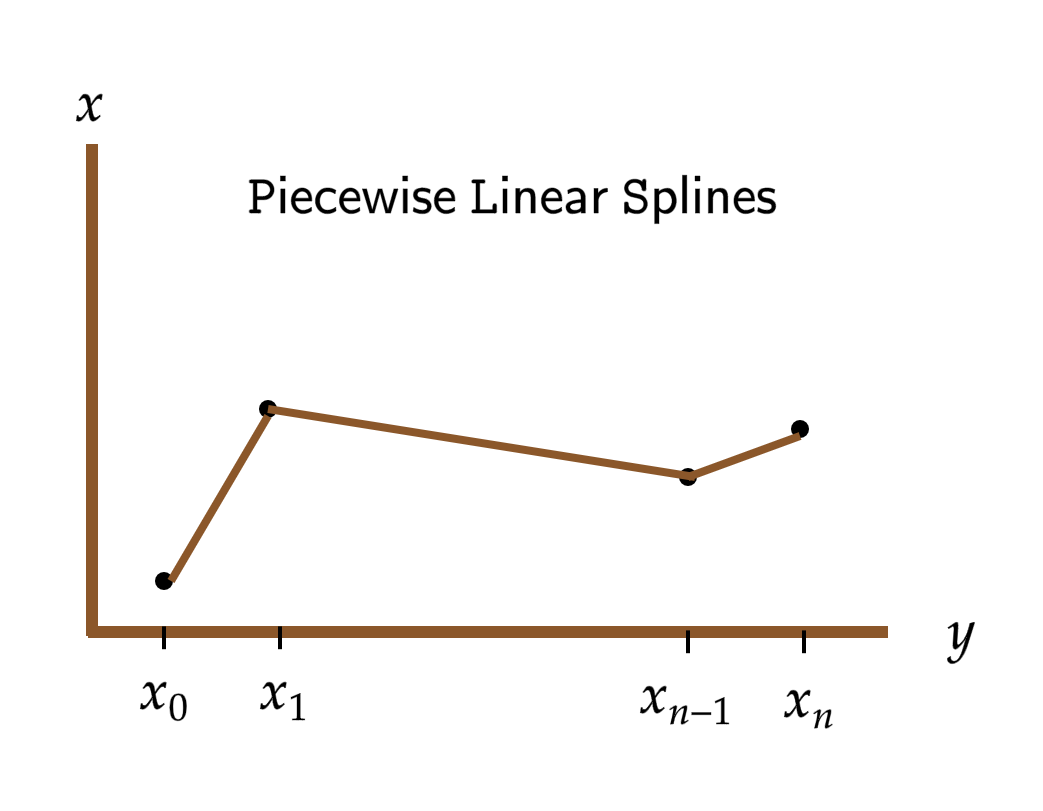
\includegraphics[width=\textwidth]{fig-17.png}
		\end{center}
	\end{marginfigure}

	\subsection{The Simplex Algorithm: Initialization}
	\begin{defn}[Auxiliary Problem]
		Given a linear program,
		\[
				\begin{array}{cc}
				\operatorname{maximize} & \sum_{j = 1}^n c_jx_j \\
				\text{ subject to } & \sum_{j=1}^{n} a_{i j} x_{j} \leq b_{i} \quad(i \in [m]) \\
				& x_{j} \geq 0 \quad(j \in [n]) 
			\end{array}
		\]
	\noindent the \textbf{auxiliary problem} is defined as,
		\[
			\begin{array}{cc}
				\operatorname{minimize} & x_{0} \\
				\text{ subject to } & \sum_{j=1}^{n} a_{i j} x_{j}-x_{0} \leq b_{i} \quad(i \in [m]) \\
				& x_{j} \geq 0 \quad(j \in [n]) 
			\end{array}
		\]
	\end{defn}

	\begin{ex}{Initialization}{label}
		The \textbf{all-zero} solution is not always feasible,
		\[
		\begin{array}{cccccccc}
		\operatorname{maximize} & x_{1} & - & x_{2} & + & x_{3} & \\
		\text { subject to } & 2 x_{1} & - & x_{2} & + & 2 x_{3} & \leq & 4 \\
		& 2 x_{1} & - & 3 x_{2} & + & x_{3} & \leq & -5 \\
		& -x_{1} & + & x_{2} & - & 2 x_{3} & \leq & -1 \\
		& & & x_{1}, & x_{2}, & x_{3} & \geq & 0
		\end{array}
		\]
	\end{ex}

	\begin{rmk}
		The original problem has a feasible solution if and only if the optimum value of the auxiliary problem is zero\footnote{We solve the auxiliary problem first.}.
	\end{rmk}


	\subsection{The Simplex Algorithm: Efficiency}
	\begin{marginfigure}
		\textbf{(Conjecture)}
		The simplex algorithm is polynomial time if, given a choice, it chooses the pivot variables at random.
	\end{marginfigure}

	\begin{thm}
		With Bland's Rule, the simplex algorithm terminates in,
		\[\binom{m+n}{m} >> 2^{m+n} \quad \text{iterations.}\]
	\end{thm}

	\begin{proof}
		This follows from the fact that there are $\binom{m+n}{m}$ bases cases, and the dictionary corresponding to each basis can only appear once.
	\end{proof}

	\begin{rmk}
		The simplex algorithm typically makes $O(m)$ pivots, where $m$ is the number of constraints\footnote{Since the number of constraints in the dual is the number of variables in the primal, $O(n)$ pivots are typically needed to solve the dual. If $n < m$, taking the dual gives a quicker solution.}.  Each pivot takes $O(mn)$ with dictionaries.
	\end{rmk}

	\subsection{Linear Programming Duality}
	\begin{thm}[Weak Duality Theorem]
		For any primal feasible solution $x$ and any dual feasible solution $y$, we have $c^Tx \leq b^Ty$.
	\end{thm}

	\begin{proof}
		Using the matrix encodings\footnote{$\geq$ applies to all entries.} of the linear programs $x$ and $y$,
		\begin{align*}
			c^T \cdot x &\leq (A^Ty)^T \cdot x \text{ since $A^{T}y \geq c$ and taking the transpose}\\
					 &= (y^TA) \cdot x \\
					 &= y^T \cdot (Ax) \\
					 &\leq y^T \cdot b \text{ by the dual feasibility of $x$}
		\end{align*}
	\end{proof}

	\begin{ex}{Duality}{label}
		Consider the primal,
		\[
			\begin{array}{cccccccccc}
			\operatorname{maximise} & 4x_{1} & + & x_{2} & + & 5x_{3} & + & 3x_{4} & & \\
			\text { subject to } & x_{1} & - & x_{2} & - & x_{3} & + & 3 x_{4} & \leq & 1
			\\ & 5 x_{1} & + & x_{2} & + & 3 x_{3} & + & 8 x_{4} & \leq & 55
			\\ & -x_{1} & + & 2 x_{2} & + & 3 x_{3} & - & 5 x_{4} & \leq & 3
			\\ & & & & x_{1}, & x_{2}, & x_{3} & , x_{4} & \geq & 0
			\end{array}
		\]
		\noindent and its dual,
		\[
		\begin{array}{ccccccccc}
		\operatorname{minimize} & y_{1} & + & 55 y_{2} & + & 3 y_{3} & &
		\\ \text { subject to } & y_{1} & + & 5 y_{2} & - & y_{3} & \geq & 4
		\\ & -y_{1} & + & y_{2} & + & 2 y_{3} & \geq & 1 \\
		& -y_{1} & + & 3 y_{2} & + & 3 y_{3} & \geq & 5
		\\ & 3 y_{1} & + & 8 y_{2} & - & 5 y_{3} & \geq & 3
		\\ & & & y_{1}, & y_{2} & y_{3} & \geq & 0
		\end{array}
		\]

		\noindent The primal has optimal solution,
		\[(x_1, x_2, x_3, x_4) = (0, 14, 0, 5) = 29\]
		\noindent The dual has optimal solution,
		\[(y_1, y_2, y_3) = (11,0,6) = 29\]
	\end{ex}

	\begin{thm}[Strong Duality Theorem]
		Let $x$ be an optimal primal solution and $y$ be an optimal dual solution\footnote{An optimal solution might not exist: \begin{itemize}
			\item The feasible region is empty
			\begin{itemize}
				\item $x_1 \leq 1$
				\item $x_2 \geq 2$
			\end{itemize}
			\item The optimal value is infinite
			\begin{itemize}
				\item $\max x_1 + x_2$
				\item $x_1, x_2 \geq 0$
			\end{itemize}
		\end{itemize}}. Then $c^Tx = b^Ty$.
	\end{thm}

	\begin{proof}
		The simplex algorithm finds the optimal primal solution. It has decision variables $(x_1^*, \cdots, x_n^*)$ and slack variables $(x_{n+1}^* \cdots, x_{n+m}^*)$. The top row of the final dictionary is,
		\[z = \texttt{OPT} - \sum_{k=1}^{n+m} \gamma_k x_k\]
		\noindent where $\gamma_k \geq 0$, with equality for basis variables. Define dual variables $y_i^* = \gamma_{n+i}$ for $i \in [m]$. We need to show that,
		\begin{enumerate}
			\item $(y_1^*, \cdots, y_m^*)$ is a feasible solution for the dual,
		\[\sum_{i=1}^m a_{ij}y_i^* \geq c_j \quad \forall j \in [n]\]
			\item The value of $(y_1^*, \cdots, y_m^*)$ is equal to the optimal primal value,
			\[\sum_{j=1}^{n} c_{j} \cdot x_{j}^{*}=\sum_{i=1}^{m} b_{i} \cdot y_{i}^{*}\]
		\end{enumerate}
		\noindent  Let $z^* = \texttt{OPT(primal)} = \sum_{j=1}^n c_j \cdot x_j^*$. The final dictionary states that,
		\begin{align*}
			z &= \sum_{j=1}^n c_j \cdot x_j^* - \sum_{k=1}^{n+m} \gamma_k \cdot x_k \\
			  &= z^* - \sum_{k=1}^{n+m} \gamma_k \cdot x_k \\
			  &= \texttt{OPT(primal)} - \sum_{k=1}^{n+m} \gamma_k \cdot x_k \\
			  &= \texttt{OPT(primal)} - \sum_{k=1}^{n} \gamma_k \cdot x_k \ - \sum_{k=n+1}^{n+m} \gamma_k \cdot x_k \\
			  &\text{Re-indexing the sum to work with the dual variables,} \\
			  &= \texttt{OPT(primal)} - \sum_{j=1}^{n} \gamma_j \cdot x_j \ - \sum_{i=1}^{m} \gamma_{n+i} \cdot x_{n+1} \\
			  &\text{Since $y_i^* = \gamma_{n+i}$ for $i \in [m]$ by definition of the optimal dual solution,} \\
			  &= \texttt{OPT(primal)} - \sum_{j=1}^{n} \gamma_j \cdot x_j \ - \sum_{i=1}^{m} y_i^* \cdot x_{n+1} \\
			  &\text{But $x_{n+i}$ are our slack variables,} \\
			  &= \texttt{OPT(primal)} - \sum_{j=1}^{n} \gamma_j \cdot x_j \ - \sum_{i=1}^{m} y_i^* \cdot \bigg(b_i - \sum_{j=1}^n a_{ij} \cdot x_j\bigg) \\
			  &\text{Re-arranging,} \\
			  &= \bigg(\texttt{OPT(primal)} - \sum_{i=1}^m b_i \cdot y_i^*\bigg) + \sum_{j=1}^n \bigg(\sum_{i=1}^m a_{ij}y_i^* - \gamma_j\bigg) \cdot x_j
		\end{align*}
		\noindent Since this equality holds for all choices of $\{x_1, \cdots x_n\}$,
		\[c_j = \sum_{i=1}^m a_{ij} \cdot y_i^* - \gamma_j\]
		\noindent But $\gamma_j \geq 0$, so we have feasibility,
		\[\sum_{i=1}^m a_{ij} \cdot y_i^* \geq c_j\]
		\noindent and it must be that,
		\[\texttt{OPT(primal)} - \sum_{i=1}^m b_i \cdot y_i^* = 0\]
		\noindent so we have strong duality,
		\[\sum_{i=1}^{m} b_{i} \cdot y_{i}^{*}=0 = \texttt{OPT(primal)}=\sum_{j=1}^{n} c_{j} \cdot x_{j}^{*}\]
	\end{proof}
	
	\begin{rmk}
		The primal is infeasible if the optimal of the dual is $-\infty$ or $\infty$.
	\end{rmk}

	\begin{thm}[Completemenary Slackness Theorem]
		TFAE,
		\begin{itemize}
			\item $x$ and $y$ are optimal solutions
			\item $c \cdot x = y \cdot b$
			\item $c \cdot x = yAx$
			\item $yAx = y \cdot b$
			\item $x$ and $y$ satisfy the complementary slackness conditions
		\end{itemize}
	\end{thm}

	\begin{proof}
		This is a result of strong duality.
	\end{proof}

	\subsection{Applications of Linear Programming}

	\begin{marginfigure}
		Linear programs can model \textbf{Boolean combinatorial circuits}. For each gate $g$, there is a variable $0 \leq x_g \leq 1$. Then,
		\begin{itemize}
			\item \texttt{INPUT} gates are set to their input

			\begin{center}
				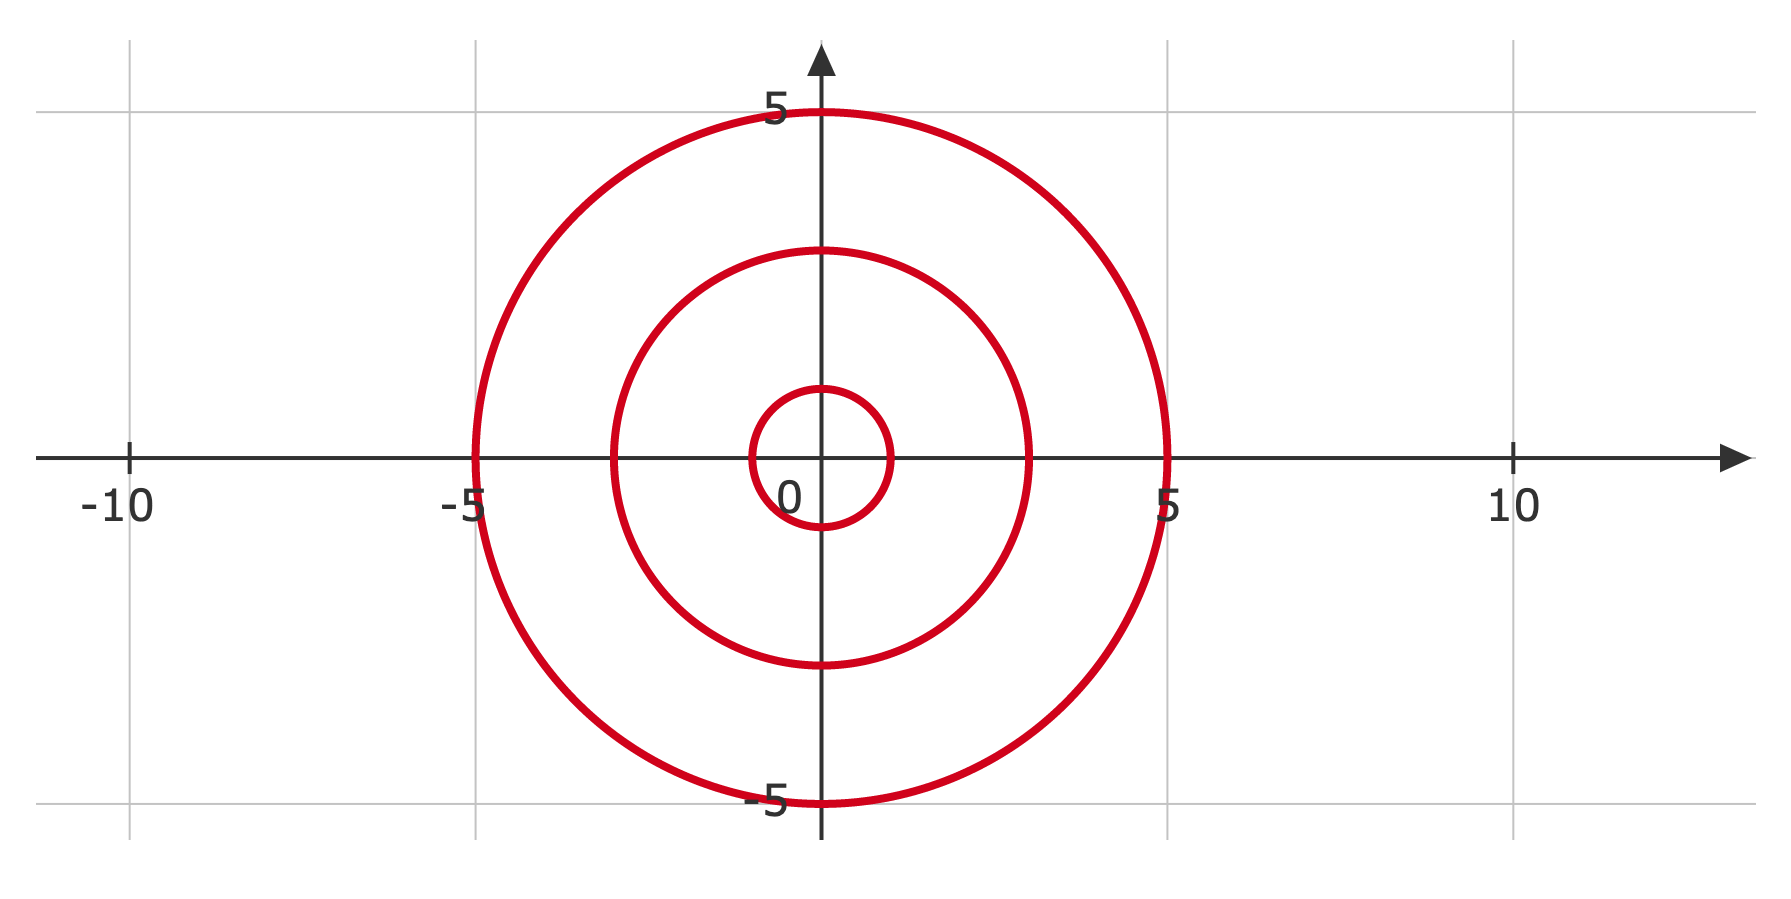
\includegraphics[width=\textwidth]{fig-5.png}
			\end{center}
			
			\item \texttt{NOT} gates are set to the opposite

			\begin{center}
				
\includegraphics[width=\textwidth]{fig-6.png}
			\end{center}
			
			\item \texttt{OR} gates are set $\max \{x_{h_1}, x_{h_2}\}$

			\begin{center}
				
\includegraphics[width=\textwidth]{fig-7.png}
			\end{center}
			
			\item \texttt{AND} gates are set to $\min \{x_{h_1}, x_{h_2}\}$

			\begin{center}
				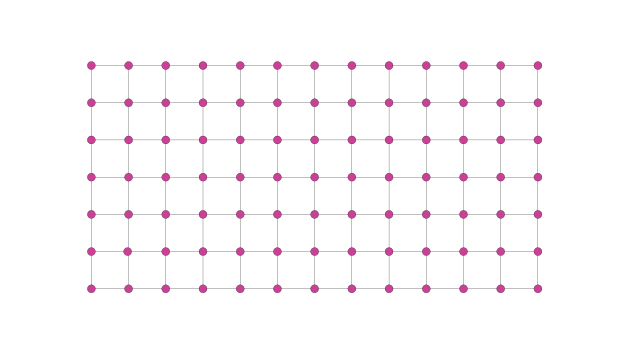
\includegraphics[width=\textwidth]{fig-8.png}
			\end{center}
			
			
		\end{itemize}
	\end{marginfigure}

	\begin{ex}{Matching as a Motivating Example}{label}
		Let $G = (V, E)$ be an undirected graph. The integer formulation of the \textbf{matching problem} is,
		\begin{itemize}
			\item An edge $e$ in the graph is picked if $x_e = 1$,
			\[x_e \in \{0,1\} \quad \forall e \in E\]
			\item We want to maximize the number of edges in the matching,
			\[\max \sum_{e \in E} x_e\]
			\item One edge is incident to each vertex,
			\[\sum_{e \in \delta(v)} x_e \leq 1 \quad \forall e \in E\]
		\end{itemize}
		\noindent In summary,
		\[
			\begin{array}{lll}
				\operatorname{maximize} & \sum_{e \in E} x_{e} & \\
				\text{ subject to } & \sum_{e \in \delta(v)} x_{e} \leq 1 & \quad \forall v \in V \\
				& x_{e} \in\{0,1\} & \quad \forall e \in E
			\end{array}
		\]
		\noindent We do not have a polynomial time algorithm for solving integer programs. If we relax the integrality constraints,
		\[
			\begin{array}{lll}
				\operatorname{maximize} & \sum_{e \in E} x_{e} & \\
				\text{ subject to } & \sum_{e \in \delta(v)} x_{e} \leq 1 & \quad \forall v \in V \\
				& x_{e} \geq 0 & \quad \forall e \in E
			\end{array}
		\]
		\noindent we may obtain a fractional solution,
		\begin{center}
			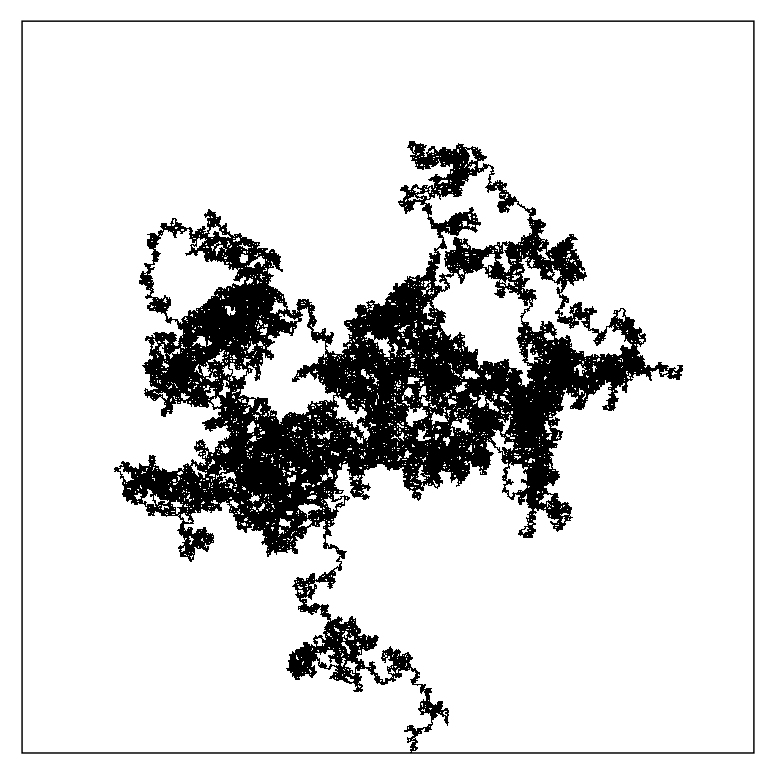
\includegraphics[width=0.45\textwidth]{fig-9.png}
		\end{center}
	\end{ex}

	\begin{marginfigure}
		Recall the following,
		\begin{itemize}
			\item The simplex algorithm outputs a basic solution, which is an extreme point of the feasible region.
			\item The feasible region is the convex hull of the extreme points.
			\item A basic solution is not a convex combination of two feasible ones.
		\end{itemize}
		\noindent where a \textbf{convex combination} is a linear combination of points where all coefficients are non-negative and sum to 1.
	\end{marginfigure}

	\begin{thm}[Bipartite Matching]
		Bipartite graphs have an optimal integral solution to the following linear program,
		\[
			\begin{array}{lll}
				\operatorname{maximize} & \sum_{e \in E} x_{e} & \\
				\text{ subject to } & \sum_{e \in \delta(v)} x_{e} \leq 1 & \quad \forall v \in V \\
				& x_{e} \geq 0 & \quad \forall e \in E
			\end{array}
		\]
	\end{thm}

	\begin{proof}
		Let $x$ be a basic solution to our linear program. We need to show that $x_e \in \{0,1\}$ for all $e \in E$. Suppose not. Then, $x_e \in (0,1)$ for all $e \in E$. If $x_e = 0$, then we can recurse on $G - \{e\}$ to produce a strictly fractional collection of $x_e$ values. Similarly, if $x_e = 1$, then we can recurse on $G - e$ since no edge adjacent to $e$ will produce a matching on this subgraph.
		\begin{itemize}
			\item \textbf{Case 1.} $G$ contains a cycle $C$.
			\begin{itemize}
				\item $C$ contains an even number of edges, and therefore we can partition $C$ into two equal sized matchings $M_1, M_2$
				\item Define two linear programs $y, z$ as follows,
				\[
				y_{e}=\left\{\begin{array}{ll}x_{e}+\epsilon & \text { if } e \in M_{1} \\ x_{e}-\epsilon & \text { if } e \in M_{2} \\ x_{e} & \text { if } e \notin C\end{array} \quad \quad z_{e}= \begin{cases}x_{e}-\epsilon & \text { if } e \in M_{1} \\ x_{e}+\epsilon & \text { if } e \in M_{2} \\ x_{e} & \text { if } e \notin C\end{cases}\right.
				\]
				\item Observe that $x$ is a convex combination of $y$ and $z$,
				\[x = \frac{1}{2} \cdot (y + z)\]
				\item Furthermore, $x$ is fractional,
				\[0 < x_e < 1 \quad \forall e \in E\]
				\item Thus, we can pick $\epsilon$ such that both $y$ and $z$ are fractional,
				\[0<y_{e}<1 \quad \forall e \in E \quad \quad \quad 0<z_{e}<1 \quad \forall e \in E\]
				\item Adding and subtracting $\epsilon$ along the red, we see that,
				\[\forall v \in V \quad \sum_{e \in \delta(v)} x_{e}=\sum_{e \in \delta(v)} y_{e}=\sum_{e \in \delta(v)} z_{e} \leq 1\]
				\item This implies that $x$ is a convex combination of two feasible solutions. Thus, $x$ is not a basic solution.
			\end{itemize}

			\item \textbf{Case 2.} $G$ is acyclic, i.e., $G$ is a forest.
			\begin{itemize}
				\item Let $P$ be a maximal path in $G$. We can partition $P$ into two matchings $P_1, P_2$ and define two linear programs $y, z$,
				\[y_{e}=\left\{\begin{array}{ll}x_{e}+\epsilon & \text { if } e \in P_{1} \\ x_{e}-\epsilon & \text { if } e \in P_{2} \\ x_{e} & \text { if } e \notin P\end{array} \quad \quad z_{e}= \begin{cases}x_{e}-\epsilon & \text { if } e \in P_{1} \\ x_{e}+\epsilon & \text { if } e \in P_{2} \\ x_{e} & \text { if } e \notin P\end{cases}\right.\]
				\item Repeating the same argument from Case 1 with $x = \frac{1}{2} \cdot (y + z)$,
				\[0<y_{e}<1 \quad \forall e \in E \quad \quad \quad 0<z_{e}<1 \quad \forall e \in E\]
				\item For any vertex $v \in V \{v_{1}, v_{2}\}$,
				\[\forall v \in V \backslash\left\{v_{1}, v_{2}\right\} \quad \sum_{e \in \delta(v)} x_{e}=\sum_{e \in \delta(v)} y_{e}=\sum_{e \in \delta(v)} z_{e} \leq 1\]
				\item $v_1$ is necessarily a leaf, meaning that it is incident to one edge,
				\[\sum_{e \in \delta\left(v_{1}\right)} y_{e}<1 \quad \sum_{e \in \delta\left(v_{1}\right)} z_{e}<1\]
				\item Since the same holds for $v_2$, $x$ is a convex combination of two feasible solutions. Thus, $x$ is not a basic solution.
			\end{itemize}
		\end{itemize}
		\noindent Hence, the optimal solution to the program is integral.
	\end{proof}

	\begin{cor}
		A similar argument shows that we can solve the \textbf{maximum weight matching problem} for bipartite graphs in polynomial time,
		\[
			\begin{array}{lll}
				\operatorname{maximize} & \sum_{e \in E} w_e \cdot x_{e} & \\
				\text{ subject to } & \sum_{e \in \delta(v)} x_{e} \leq 1 & \quad \forall v \in V \\
				& x_{e} \geq 0 & \quad \forall e \in E
			\end{array}
		\]
	\end{cor}

	\begin{marginfigure}
		$A$ is the incidence matrix, 
		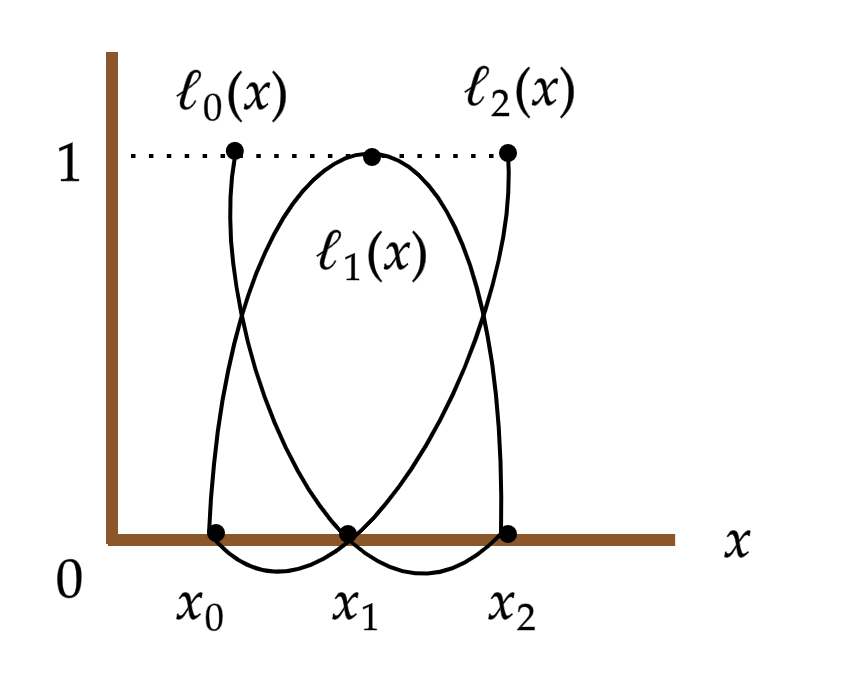
\includegraphics[width=0.8\textwidth]{fig-10.png}
	\end{marginfigure}

	\begin{rmk}
		The matrix encoding of the dual linear program is,
		\[
		   \min \underbrace{\Set{ 1^Ty \ | \begin{array}{l}
		    A^T y \geq c \\
		    y \geq 0
		  \end{array}}}_{Dual}
			\iff
			\max \underbrace{\Set{ 1^Tx \ | \begin{array}{l}
		    Ax \leq 1 \\
		    x \geq 0
		  \end{array}}}_{Primal}
		\]
		\noindent allowing us to re-interpret the dual as the \textbf{vertex cover problem},
		\[
		\begin{array}{lll}
				\operatorname{minimize} & \sum_{v \in V} y_v & \\
				\text{ subject to } & y_u + y_v \geq 1 & \quad \forall (u,v) \in E \\
				& y_v \geq 0 & \quad \forall v \in V
			\end{array}
		\]
	\end{rmk}

	\begin{ex}{The Shortest Path Problem}{label}
		Given a directed graph $G = (V, A)$ with a source vertex $s$ and a sink vertex $t$, we can set up the shortest path problem,
		\begin{itemize}
			\item Let each arc $a \in A$ have non-negative length $l_a$
			\item The length of a path $P$ is,
			\[l(P) = \sum_{a \in P}l_a\]
		\end{itemize}
		We can formulate this as an \textbf{integer program},
		\[
		\begin{array}{ll}
				\operatorname{minimize} & \sum_{a \in A} \ell_{a} \cdot x_{a} \\
				\text{ subject to } & x_{a} \in\{0,1\} \quad \forall a \in A \\
				& \sum_{a \in \delta^{-}(v)} x_{a}-\sum_{a \in \delta+(v)} x_{a}= \begin{cases}-1 & v=s \\
												0 & v \neq\{s, t\} \\
												1 & v=t\end{cases}
			\end{array}
		\]
		\noindent and do a constraint relaxation.
	\end{ex}

	\begin{thm}[Shortest Path]
		The shortest path problem has an optimal integral solution to the following linear program,
		\[
		\begin{array}{ll}
				\operatorname{minimize} & \sum_{a \in A} \ell_{a} \cdot x_{a} \\
				\text{ subject to } & x_{a} \geq 0 \quad \forall a \in A \\
				& \sum_{a \in \delta^{-}(v)} x_{a}-\sum_{a \in \delta+(v)} x_{a}= \begin{cases}-1 & v=s \\
												0 & v \neq\{s, t\} \\
												1 & v=t\end{cases}
			\end{array}
		\]
	\end{thm}

	\begin{proof}
		Any basic solution $x$ represents an $(s-t)$ flow of value $1$. By the Flow Decomposition Theorem, $x$ decomposes into $(s,t)$ paths,
		\begin{align*}
			&\mathbf{x}=\alpha_{1} \cdot P_{1}+\alpha_{2} \cdot P_{2}+\cdots+\alpha_{k} \cdot P_{k} \\
			&\text{where } \sum_{i=1}^{k} \alpha_{i}=1 \text{ and } \alpha_{i} \geq 0 \quad \forall i
		\end{align*}
		\noindent 
	\end{proof}
	\noindent but each $P_i$ is a feasible solution to the linear program. Either we have a contradiction, or $k = 1$. If $k = 1$, then $x$ is an $(s-t)$ path itself and is an integral solution.

	\begin{marginfigure}
		$A_{ij}$ is negative if $v_i$ is the tail of $a_j$,
		
\includegraphics[width=0.8\textwidth]{fig-11.png}
	\end{marginfigure}

	\begin{rmk}
		The matrix encoding of the dual linear program, even though the primal is not in standard form, is,
		\[\max \Set{ y_t - y_s \ | \begin{array}{l}
		    y_v \text{ unrestricted } \quad \forall v \in V  \\
		    A^Ty \leq l
		  \end{array}}\]
		\noindent Changing labels of $y$ to $d$ to represent distances,
		\[\max \Set{ d_t - d_s \ | \begin{array}{l}
		    d_v \text{ unrestricted } \quad \forall v \in V  \\
		    d_v - d_u \leq l_{uv} \quad \forall a = (u,v) \in A
		  \end{array}}\]
		\noindent setting $d_s = 0$, we see that $d_v$ is the distance from $v$ to $s$.
	\end{rmk}

	\begin{ex}{Maximum Flow Problem}{label}
		Recalling our formulation of maximum flow,
		\[
		\begin{array}{ll}
				\operatorname{maximize} & \sum_{a \in \delta^-(t)} f_{a} \\
				\text{ subject to } & 0 \leq f_a \leq u_a \quad \forall a \in A \\
				& \sum_{a \in \delta^{-}(v)} f_{a} = \sum_{a \in \delta^{+}(v)} f_{a} \quad \forall v \in V - \{s,t\}
			\end{array}
		\]
	\end{ex}

	\begin{ex}{Zero-Sum Games}{label}
		The \textbf{Minimax Theorem} is a result of the linear programming duality. It states that for any matrix $A$,
		\[\max _{\mathbf{x}}\left[\min _{\mathbf{y}} \mathbf{x}^{T} A \mathbf{y}\right]=\min _{\mathbf{y}}\left[\max _{\mathbf{x}} \mathbf{x}^{T} A \mathbf{y}\right]\]
	\end{ex}